\section{Szögsebesség szabályozás állapotvisszacsatolással}

%{{{ Pólusok számítása
\subsection{Pólusok számítása}

Írjuk át a rendszerünket állapotteres alakra, valamint a $\fn{W}_\text{c}$ kontrollert
cseréljük le a $\mathrm{K}_\text{x}$, $\mathrm{K}_\text{rx}$ és $\mathrm{K}_\text{ru}$ állapotvisszacsatoló és
alapjelkompenzáló mátrixokra.
A $\B{D}$ és $\B{K}_\text{rx}$ mátrix esetünkben zérus, és $\B{K}_\text{ru}$ egységnyi.

\begin{figure}[H]
    \centering
    \incfig[.8\textwidth]{5a_allapotter_hatasvazlat}
    \caption{Állapottér modell hatásvázlata}
    \label{fig:5a_allapotter_hatasvazlat}
\end{figure}

A rendszer átviteli függvény formában van megadva:
\begin{equation}
	\fn{W}_\text{p} = \frac{\Psi}{(1+T_1s)(1+T_2s)} = \frac{\Psi}{T_1T_2s^2+(T_1+T_2)s+1} = 
	\frac{\frac{\Psi}{T_1T_2}}{s^2+\frac{T_1+T_2}{T_1T_2}s+\frac{1}{T_1T_2}}.
\end{equation}

Írjuk át ezt állapottér modellre, irányíthatósági kanonikus alakra:
\begin{equation}
	\fn{Y} = \frac{\frac{\Psi}{T_1T_2}}{s^2+\frac{T_1+T_2}{T_1T_2}s+\frac{1}{T_1T_2}}\fn{U}
\end{equation}
\begin{equation}
	\fn{X} := \frac{1}{s^2+\frac{T_1+T_2}{T_1T_2}s+\frac{1}{T_1T_2}}\fn{U}\,\Rightarrow
\end{equation}
\begin{equation}
	u = \ddot{x} + \frac{T_1+T_2}{T_1T_2}\dot{x} + \frac{1}{T_1T_2}x\,\Rightarrow
\end{equation}
\begin{equation}
	\underbrace{\mat{\dot{x}\\\ddot{x} }}_{\dot{\B{x} }}
	= \underbrace{\mat{0&1\\-\frac{1}{T_1T_2}&-\frac{T_1+T_2}{T_1T_2} }}_{\B{A}}
	\underbrace{\mat{x\\\dot{x} }}_{\B{x}}
	+ \underbrace{\mat{0\\1}}_{\B{B}}\B{u}
\end{equation}
\begin{equation}
	\B{y} = \underbrace{\mat{\frac{\Psi}{T_1T_2}&0}}_{\B{C}}\mat{x\\\dot{x}} + \underbrace{\mat{0}}_{\B{D}}\B{u}
\end{equation}

A feladatkiírás alapján a domináns időállandó $\widetilde{T}_1=50~\text{ms}~=0,05$ s
kell hogy legyen.

Az átviteli függvény karakterisztikus egyenlete legyen adott a következő alakban
\begin{equation}
	\fn{p}(s) = s^2 + a_1 s + a_0 s.
\end{equation}
A túllövés a $\xi$ csillapítástól függ, amelyek adottak, így ki tudjuk számítani a
kívánt $a_1$ és $a_0$ együtthatókat.
\begin{align}
	\widetilde{T}_1 &= \sqrt{\frac{1}{a_0}}\,\Rightarrow a_0 = 400\\
	\Delta v        &= 0,1 = \operatorname{exp}\brc{\frac{-\xi\pi}{\sqrt{1-\xi^2}} }
	\,\Rightarrow \xi = 0,5911\\
	\xi             &= \frac{a_1}{2\sqrt{a_0}}\,\Rightarrow a_1 = 23,6462
\end{align}
% W = b0 / (a2*s^2 + a1*s + a0)
% T = sqrt(a2/a0)
% xi = a1 / (2*sqrt(a0*a2))
% dv = exp(-xi*pi / sqrt(1-xi^2))
%
Tehát \fbox{$a_0 = 400$ és $a_1 = 23,65$}.


%}}}

%{{{ A szabályozó mátrix számítása
\subsection{A szabályozó mátrix számítása}


A visszacsatolás miatt
\begin{equation}
	\B{u} = \B{r} - \B{K}_\text{x}\B{x}
\end{equation}
\begin{equation}
	\dot{\B{x}} = \B{A}\B{x} + \B{B}\B{r} - \B{B}\B{K}_\text{x}\B{x}
\end{equation}
\begin{equation}
	\dot{\B{x}} = \brc{\B{A}-\B{B}\B{K}_\text{x}}\B{x} + \B{B}\B{r}
\end{equation}
Ebben a feladatrészben  tehát a referencia bemenetre nézve
a bemeneti mátrix nem változik, az új rendszermátrix pedig $\widetilde{\B{A}} = \B{A}-\B{B}\B{K}_\text{x}$.
A $\B{K}_\text{x}$ mátrixot a kívánt pólusok alapján kell megválasztani a következőképpen.
a kívánt pólusok legyenek.

\begin{equation}
	\widetilde{\fn{p}}(s) = s^2 + a_1s + a_0
\end{equation}

\begin{equation}
	\widetilde{\B{A}} = \mat{0&1\\-\frac{1}{T_1T_2}&-\frac{T_1+T_2}{T_1T_2}} - 
	\mat{0&0\\k_1&k_2} = \mat{0&1\\-\frac{1}{T_1T_2}-k_1&-\frac{T_1+T_2}{T_1T_2}-k_2} = 
	\mat{0&1\\ -a_0& -a_1}
\end{equation}

Ebből a keresett mátrix
\begin{equation}
	\B{K} = \mat{k_1&k_2} = \mat{-4,98\cdot10^5& -7278,6}.
\end{equation}

%}}}

%{{{ Ugrásfüggvény
\subsection{Ugrásfüggvény}

Az üresjárati szögsebesség $\omega_\text{noload} = 5860\text{ rpm} = 932.648~\frac{\text{rad}}{\text{s}}$. Az ugrásválaszt a rendszermátrixok ismeretében a MATLAB \verb|step| függvénye rajzolja ki.

\begin{figure}[H]
	\centering
	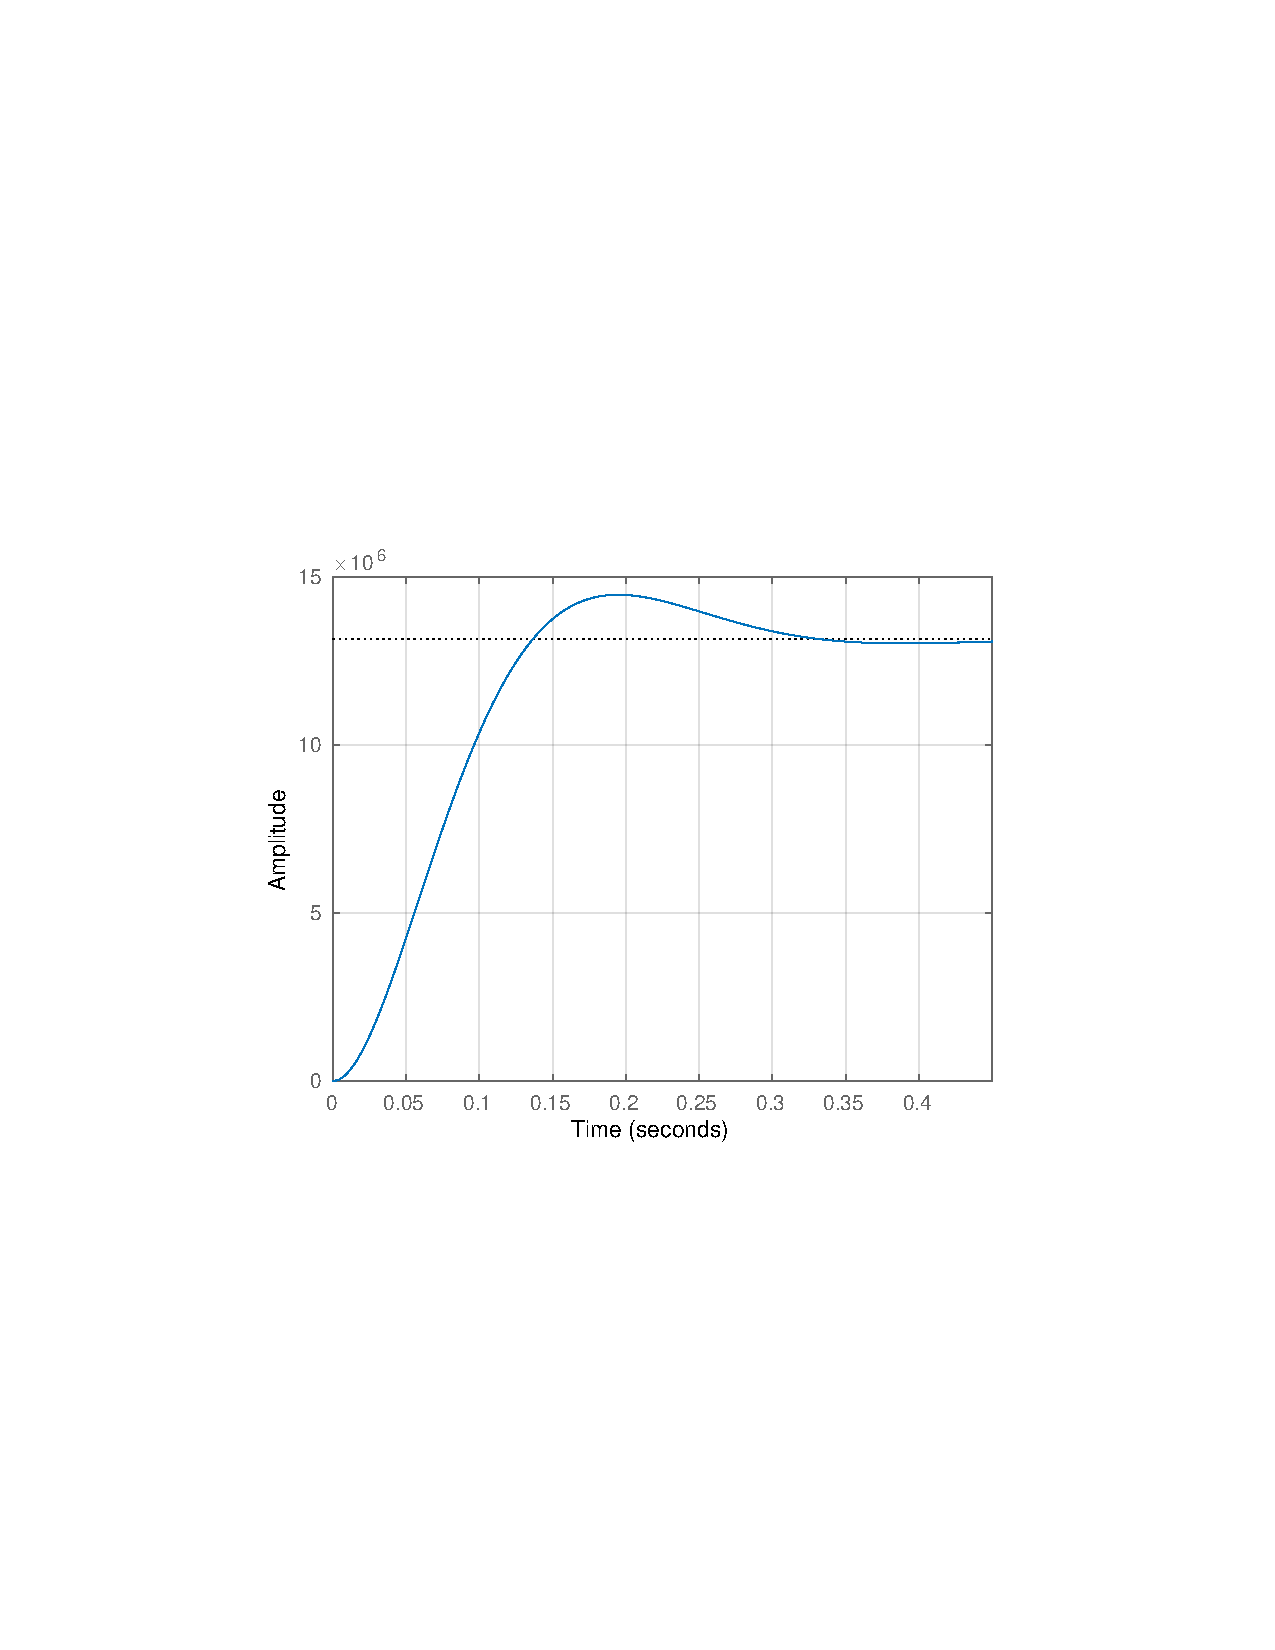
\includegraphics[width=.8\textwidth, trim=100 240 80 252, clip]{5c_step}
	\caption{A rendszer ugrásválasza}
	\label{fig:5c_step}
\end{figure}


%}}}

%{{{ Állandósult érték
\subsection{Állandósult érték}\label{subsec:5d}

Az állapottér rendszerünket írjuk vissza MATLAB segítségével átviteli függvény
alakra ($\fn{W}_\text{cl}$), amivel könnyen tudunk állandósult értéket számolni.
A bemenet legyen $\fn{X} = \frac{\omega_\text{noload}}{s}$, a rendszer válasz $\fn{Y} = \fn{W}_\text{cl}\fn{X}$.

A végérték-tétel alapján az állandósult szögsebesség $\omega_\infty = \lim\limits_{s\rightarrow 0}s\fn{Y} = 2\cdot10^7$.%TODO

%}}}

%{{{ Alapkompenzáció számítása
\subsection{Alapkompenzáció számítása}

Ha nincs statikus alapjelkompenzáció, vagyis $\B{K}_\text{rx}\equiv0$, akkor éljünk
a $\B{K}_\text{ru}:=\B{K}_\text{r}$ jelöléssel, az érthetőség kedvéért.

Most állítsuk be a $\B{K}_\text{r}$ mátrixot úgy, hogy
$\lim\limits_{t\rightarrow\infty}\B{y}=\B{r}$ igaz legyen.
Ezt a következő összefüggés adja meg:

\begin{equation}
	\B{K}_\text{r} = -\brc{\B{C}\widetilde{\B{A}}^{-1}\B{B}}^{-1} = \mat{4,6684\cdot10^{-5}}.
\end{equation}

%}}}

%{{{ Alapjelkompenzált ugrásválasz
\subsection{Alapjelkompenzált ugrásválasz}

\begin{figure}[H]
	\centering
	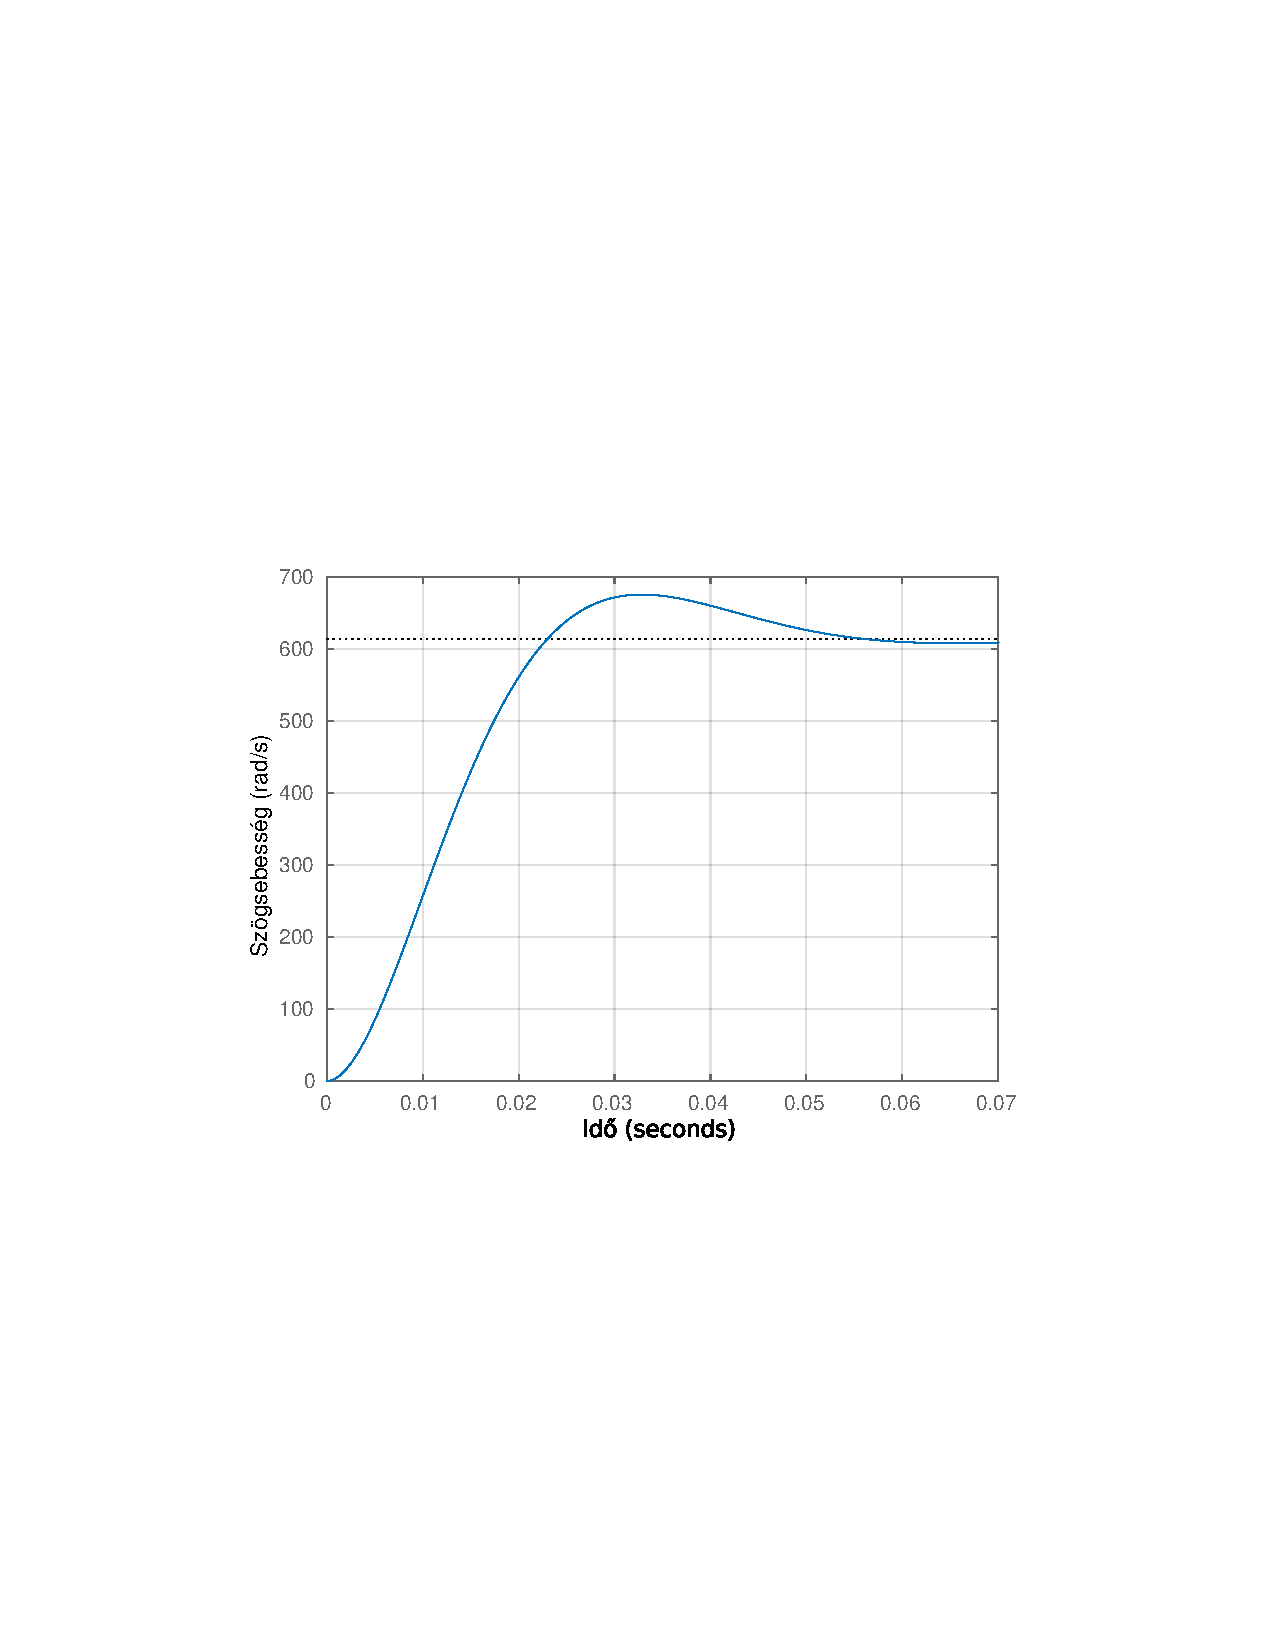
\includegraphics[width=.7\textwidth, trim=100 240 80 252, clip]{5f_step}
	\caption{A rendszer ugrásválasza alapjelkompenzálóval}
	\label{fig:5f_step}
\end{figure}

%}}}

%{{{ Állandósult érték
\subsection{Állandósult érték}

\Aref{subsec:5d}. részfeladathoz hasonló módon járunk el.
A végérték-tétel alapján az állandósult szögsebesség $\omega_\infty = \lim\limits_{s\rightarrow 0}s\fn{Y} = 932,648$.%TODO

%}}}

%{{{ Statikus alapjelkompenzáció
\subsection{Statikus alapjelkompenzáció}

Most legyen $\B{K}_\text{rx}$ nullától különböző.
Ekkor
\begin{equation}
	\mat{\B{K}_\text{rx}\\\B{K}_\text{ru}}=\mat{\B{A}&\B{B}\\\B{C}&\B{D}}^{-1}\mat{\B{0}\\\B{I}}
	= \mat{1,17\cdot10^{-7}\\0\\0,0582}.
\end{equation}

%}}}

%{{{ Statikus alapjelkompenzált ugrásválasz
\subsection{Statikus alapjelkompenzált ugrásválasz}

Írjuk fel a rendszer átviteli függvényét $\B{r}$-től $\B{y}$-ig.
\begin{align}
	\B{u} &= \brc{\B{K}_\text{ru}+\B{K}_\text{x}\B{K}_\text{rx}}\B{r} - \B{K}_\text{x}\B{x}\\
	\B{x} &= \frac{1}{s}\brc{\B{B}\B{u} + \B{A}\B{x}}\\
	\B{x} &= \frac{1}{s}\brc{\B{B}\brc{\B{K}_\text{ru}+\B{K}_\text{x}\B{K}_\text{rx}}\B{r}+\brc{\B{A}-\B{B}\B{K}_\text{x}}\B{x}}\\
	\B{x} &= \brc{\B{I}-\frac{1}{s}\brc{\B{A}-\B{B}\B{K}_\text{x} }}^{-1}\frac{1}{s}\B{B}\brc{\B{K}_\text{ru}+\B{K}_\text{x}\B{K}_\text{rx}}\B{r}\\
	\B{y} &= \B{C}\B{x} = \fbox{$\frac{400}{s^2 + 23,646 s + 400}$}
\end{align}

Az egységugrás válasz ebből a szokásos módon számítható.
\begin{figure}[H]
	\centering
	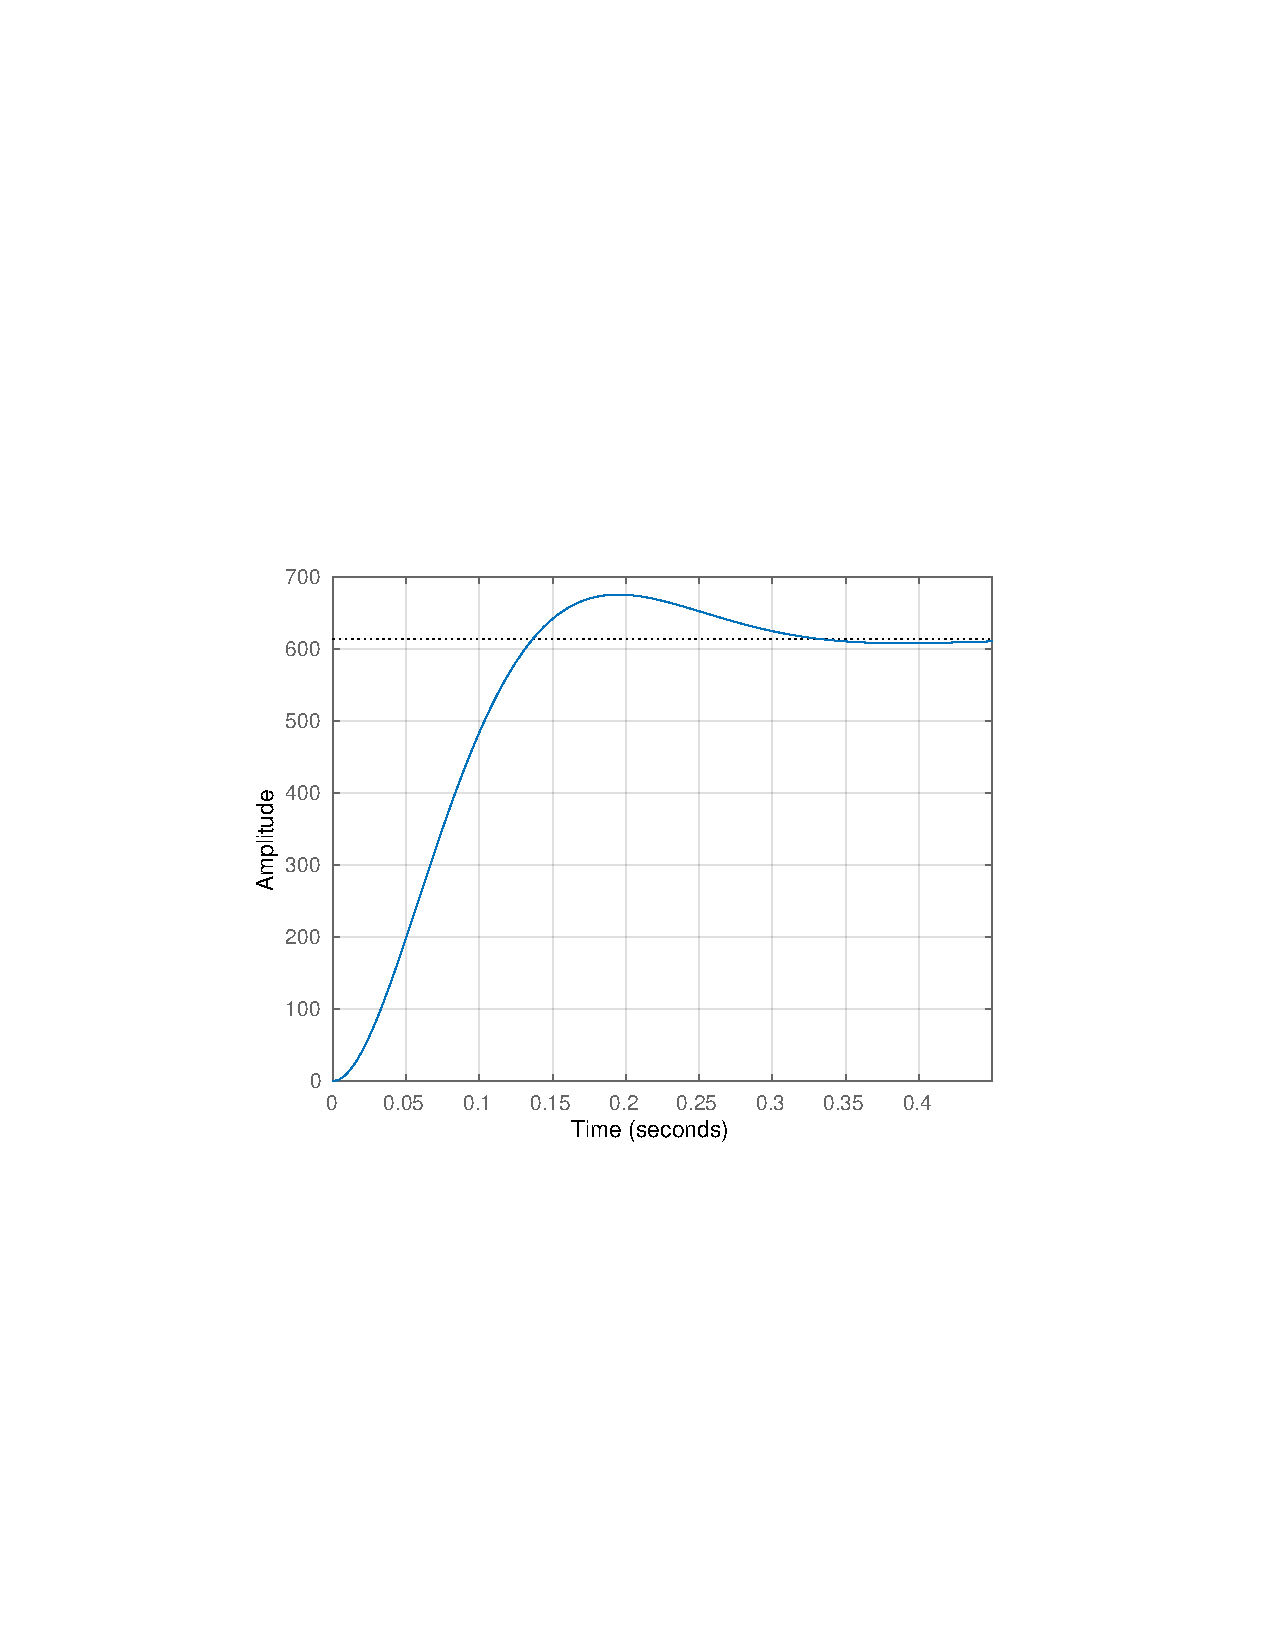
\includegraphics[width=.7\textwidth, trim=100 240 80 252, clip]{5i_step}
	\caption{A rendszer ugrásválasza statikus alapjelkompenzálóval}
	\label{fig:5i_step}
\end{figure}

%}}}

%{{{ Állandósult érték
\subsection{Állandósult érték}

A végérték-tétel alapján az állandósult szögsebesség $\omega_\infty = \lim\limits_{s\rightarrow 0}s\fn{Y} = 932,648$.

%}}}
